\documentclass[a4paper]{llncs}
\usepackage[T1]{fontenc}
\usepackage[utf8]{inputenc}
\usepackage{lmodern}

\usepackage{url}
\usepackage{graphicx}
% \usepackage{hyperref}
\usepackage{color}
\usepackage[textsize=tiny]{todonotes}

\newcommand{\ioanna}[1]{\todo[color=red]{Ioanna: #1}}
\newcommand{\mariaesther}[1]{\todo[color=cyan]{Maria-Esther: #1}}
\newcommand{\christoph}[1]{\todo{Christoph: #1}}
       
\urldef{\mails}\path|{lytra, vidal, langec, auer}@cs.uni-bonn.de|

% squeeze some space
\setlength{\parskip}{0cm}
\def\baselinestretch{0.99}
\setlength{\intextsep}{8pt}
\setlength{\abovecaptionskip}{3pt}
\setlength{\belowcaptionskip}{-10pt}

\begin{document}
	
	\mainmatter
	\title{WDAqua: Answering Questions using Web Data\thanks{The authors of this abstract are the coordinators of the project.}}
	
	\author{Ioanna Lytra, Maria-Esther Vidal, Christoph Lange \and S{\"o}ren Auer}
	\institute{University of Bonn, Germany\\ \mails\\}
	
	\maketitle
	
	\section{WDAqua in a Nutshell} \label{sec:intro}
	WDAqua, a Marie Sk{\l}odowska Curie Innovative Training Network (ITN) running from January 2015 to December 2018, involves six academic partners\footnote{University of Bonn, Fraunhofer Institute for Intelligent Analysis and Information Systems IAIS, Germany; National and Kapodistrian University of Athens, Greece; Universit{\'e} Jean Monnet Saint-{\'E}tienne, France; University of Southampton, Open Data Institute (ODI), UK.}, and employs 15 PhD students in total.
        The main motivation of this project is that sharing, connecting, analyzing, and understanding data on the Web can provide better services to citizens, communities, and the industry.
        A vehicle to achieve this is data-driven question answering (QA), having the key objective of delivering precise and comprehensive answers to natural language questions primarily by making better use of data.
        Powerful QA tools promise to improve access to the large amount of information available on the Web, or even private data collections, and can be immediately useful to a wide audience of end users in their private and professional life.
        Data-driven QA comprises four simplified steps: 1) understanding a human question, and turning it into natural language text, 2) analyzing the question in natural language, 3) finding data to answer the question and to justify the answer, and finally, 4) presenting the answer using, e.g., verbalization, natural language synthesis, or visualization.
	
	\section{Project Progress and Dissemination} \label{sec:progress}
	The aim of the WDAqua project is to advance the state of the art in the challenging research field of data-driven QA by interleaving training, research, and innovation.
        The first project year focused on the first two goals, while \christoph{Please think about this once more.  \emph{Exploitation} will happen in a late phase only, but even from the very start our work should of course be \emph{innovative} already.}innovation is expected to be achieved at the final stage of the project with the combination of the respective research results into an open data-driven QA platform and ecosystem.
	\christoph{Not quite yet, but let's claim so and hope it'll be done by ESWC.}Recruitment of the PhD students has now been completed and various research and training events have been organized by the WDAqua members.
        In particular, the 1st WDAqua Learning Week in summer 2015 was an opportunity for the participants to gain hands-on experience on different components of QA systems and establish collaborations with fellow WDAqua early stage researchers.
        Other activities include the organization of the Web Intelligence Summer School (2015), the Annual Meetup of the Question Answering Community in Germany and beyond (2015), and the organization of the 3rd International Workshop on Dataset PROFiling and fEderated Search for Linked Data (2016) at ESWC 2016.
	For training purposes, a few short-term inter-sectoral secondments among partners have been completed and more are planned for the upcoming years.
	
	At this early stage of the WDAqua research project, the researchers focused, first of all, on identifying and investigating open research questions in data-driven QA, analyzed the state of the art regarding these open challenges, and published or submitted for publication some initial results at high-quality research venues (ICSC 2016, ESWC 2016, etc.).
	The research questions the PhD students are currently working on can be classified into four key research areas strongly related to data-driven QA (\christoph{To save more space we could even have a figure without a caption and refer to it as ``\emph{the} figure'' – in a 2-page paper that's OK.}cf.\ Fig.~\ref{fig:figure}): dataset discovery (i.e., quality-driven dataset discovery and retrieval, research on collaborative knowledge bases to support question answering, handling evolution of Web data through extraction of facts in free text, trust and provenance in the Web of data), data management (making datasets fit for QA, dataset profiling, summarization, and ranking), AI and NLP approaches (translating natural language questions in queries, spoken question recognition and interpretation, data-driven text generation), and human-data interaction (interactive interlingual QA systems, challenges connected to data search and use).
        Apart from that, the project is concerned with designing the architecture of an open QA platform, to enable the integration of the different QA components that will be developed by the partners of WDAqua and beyond.
	\begin{figure}[htpb!]
	    \centering
	    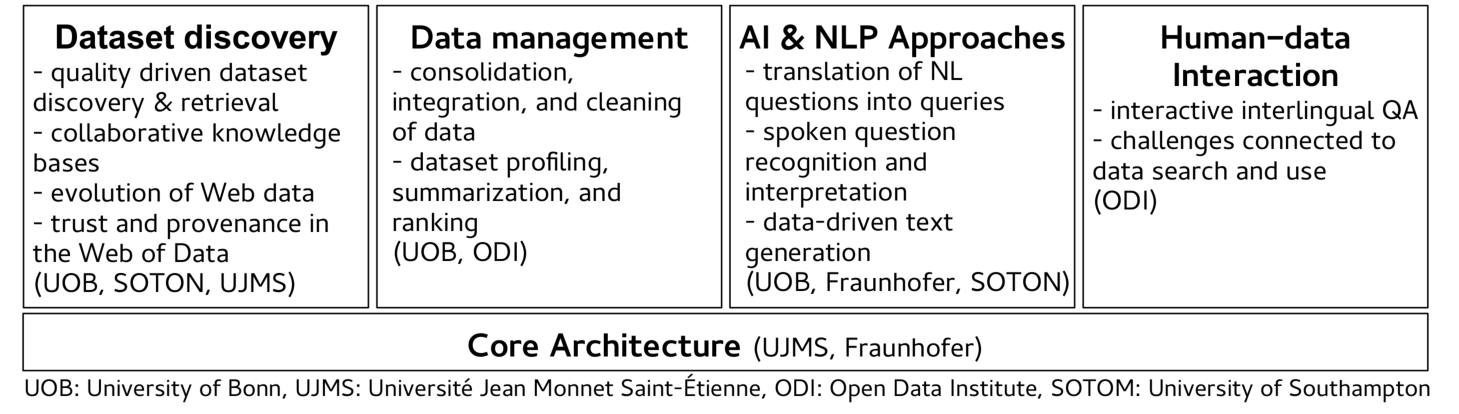
\includegraphics[width=\textwidth]{figure.pdf}
		\caption{Research challenges related to data-driven QA}
		\label{fig:figure}
	\end{figure}

	\section{Networking} \label{sec:networking}
	The WDAqua ITN aims at reaching out to the scientific community, industry, and society.
        The first steps in pursuing challenging research questions in this promising research area have been conducted and efforts have been invested in attracting input by the community, by presenting WDAqua at European and international research venues, as well as in transferring expertise to and exchanging experience with the research community by organizing training events (i.e., summer schools, learning weeks) and establishing collaborations with the industry (e.g., through internships of PhD students).
	
\end{document}
%  LocalWords:  WDAqua Ioanna Lytra ren Auer Sk odowska ITN IAIS ODI
%  LocalWords:  Fraunhofer Kapodistrian Universit Monnet tienne QA
%  LocalWords:  Meetup PROFiling fEderated ESWC sectoral ICSC NLP
%  LocalWords:  summarization interlingual
